\chapter{MTR-Eval：基准质量评估方法}

\label{chap:method2}



\section{设计动机与核心思想}

在第三章的形式化分析中，本文已明确指出：现有对话检索基准的评估失效，根本源于标注金标文档集 $G_i$ 与语料库中客观存在的真实支持文档集 $\hat{G}_i$ 之间的质量鸿沟。传统评估范式隐含了一个强假设，即 $G_i \equiv \hat{G}_i$。然而，受限于人工标注的“局部视野”与自动化合成的“静态启发式”，这一假设在现实中往往不成立。若直接基于存在缺陷的 $G_i$ 计算 Recall、NDCG 等指标，不仅无法客观反映检索模型的真实能力，反而可能因标注噪声（$G_i \setminus \hat{G}_i \neq \emptyset$）导致模型性能被高估，或因标注稀疏性（$\hat{G}_i \setminus G_i \neq \emptyset$）导致先进模型遭受假阴性惩罚。



面对包含数百万文档的工业级语料库，通过全量人工重新标注以逼近 $\hat{G}_i$ 在时间与经济成本上均不可行。为此，本文提出 MTR-Eval（如~\ref{fig:mtr-eval-framework}所示），一套基于异构大语言模型集成裁判的基准质量自动化审计方法。其核心思想在于：将难以直接枚举的真实证据集 $\hat{G}_i$ 的逼近问题，转化为一系列可计算、可验证的代理任务。通过引入细粒度的四维评估指标体系，MTR-Eval 能够在无需人工复核的前提下，动态量化基准数据集中的噪声比例与稀疏程度，并输出数据集的“可靠性系数”。该方法不仅为历史基准提供“去偏重打分”能力，更为后续高保真合成流水线（MTR-Pipeline）的质量控制提供了可微分的优化目标。



\begin{figure}[h]

    \centering

    \includegraphics[width=\linewidth]{assets/figs/mtr-eval-framework.png}

    \bicaption{MTR-EVAL审计流程}{The MTR-EVAL auditing process}
    \label{fig:mtr-eval-framework}

\end{figure}


\section{四维评估指标体系}



如第三章第\ref{sec:framework_overview}节所述，MTR-Eval 构建了覆盖"查询-文档-答案"全链路的四维评估体系，旨在从概念层面解耦基准数据中的噪声、稀疏性、幻觉与语言质量。需要强调的是，本节四维指标用于诊断基准数据本身的质量（即 $G_i$ 是否逼近 $\hat{G}_i$），而非评估检索模型在给定基准上的性能（即 $\mathcal{R}_i$ 与 $G_i$ 的重合程度），两者在评估对象、数学基础与使用阶段上均存在本质区别。本节将对这四个指标进行严格的形式化定义，并详细阐述其计算协议、评分量规与大语言模型裁判交互流程。

\subsection{查询-证据对齐度}



该指标旨在检测基准数据集中是否存在标注噪声，即金标文档集 $G_i$ 中是否混入了实际上无法回答查询 $q_i$ 的文档。从集合论角度，这直接对应于检测 $G_i \setminus \hat{G}_i \neq \emptyset$ 的情况。



形式化定义。对于评估实例 $(H_i, q_i, G_i)$ 中的任意金标文档 $d \in G_i$，该指标严格评估 $d$ 是否真正包含回答 $q_i$ 所需的充分信息。形式化地，我们定义对齐度判定逻辑如下：

\begin{equation}
    d \in G_i \setminus \hat{G}_i \iff \text{Support}(q_i, d) = \text{False}
\end{equation}

若评估模型判定 $d$ 无法支撑 $q_i$，则表明该标注为假阳性（False Positive），即基准中混入了不相关或弱相关的文档片段。该维度的低分直接揭示了基准数据集的标注噪声水平，是衡量基准纯净度的首要指标。



评估协议。评估模型被直接呈现查询 $q_i$ 与金标文档 $d$，要求判断 $d$ 是否可回答 $q_i$。采用五分制评分方法，评分从“完全不可回答”至“完全可回答”。模型必须提供显式推理链，明确指出文档中支持或反驳查询的关键句子。



\subsection{证据完备性}



该指标专为量化标注稀疏性而设计，旨在检测语料库 $\mathcal{D}$ 中是否存在未被纳入金标文档集 $G_i$ 的有效支撑文档。从集合论角度，这对应于量化 $\hat{G}_i \setminus G_i$ 的规模。由于在大规模语料库中穷举所有相关文档属于组合爆炸问题，本文采用判别性测试作为代理任务。



形式化定义。传统评估假设 $G_i$ 是完备的，但这一假设在开放域语料中往往不成立。为检测这一缺陷，我们构造候选文档池 $\mathcal{C}$如下：
\begin{equation}
    \mathcal{C} = \{d_{\text{gold}}\} \cup \{d_{\text{neg}}^{(1)}, d_{\text{neg}}^{(2)}, \dots, d_{\text{neg}}^{(k)}\}, \quad \text{其中 } d_{\text{gold}} \in G_i
\end{equation}
其中 $\{d_{\text{neg}}^{(j)}\}$ 为通过强检索器召回的困难负例。评估模型被要求从 $\mathcal{C}$ 中识别最相关文档。若模型一致性地选择非金标文档 $d_{\text{other}} \notin G_i$ 作为最优匹配，则强有力地证明语料库中存在未被标注者发现的有效证据。其简单公式表示如下：
\begin{equation}
    \text{LLM}(\mathcal{C}, q_i) = d_{\text{other}} \notin G_i \implies \hat{G}_i \setminus G_i \neq \emptyset
\end{equation}

该指标惩罚那些“金标文档并非唯一或最优匹配”的基准实例，直接反映数据构建过程中的全局视野缺失。



评估协议。在判别性测试中，文档位置经过随机化以消除位置偏差。模型需输出选择理由并明确引用支撑句子。完备性评分反映了金标文档在语义相关性上相对于未标注文档的竞争优势。



\subsection{答案-证据忠实度}



在多轮对话基准构建中，标注者或生成模型可能在未充分锚定证据的情况下直接输出答案，导致“答案-证据”脱节，即产生标注幻觉。该指标独立于检索过程，专门评估生成的答案 $a_i$ 是否严格基于 $G_i$ 生成。



形式化定义。形式化地，该指标验证答案 $a_i$ 是否完全扎根（fully grounded）于其对应的金标文档集 $G_i$。我们定义忠实度判定逻辑如下所示：
\begin{equation}
    \text{Faithful}(a_i, G_i) \iff \forall c \in \text{Claims}(a_i), \ c \subseteq G_i
\end{equation}
其中 $\text{Claims}(a_i)$ 表示答案中可独立验证的语义单元。若存在任意声明 $c$ 无法在 $G_i$ 中找到直接依据，或与 $G_i$ 陈述相矛盾，则判定为幻觉。该指标确保基准答案具备可追溯性与事实严谨性。



评估协议。裁判模型需逐句审查 $a_i$，验证其中的实体、数值与逻辑关系是否均可在 $G_i$ 中溯源。采用五分制量表进行细粒度刻画，以区分“完全忠实”至“完全不忠实”的过渡状态。



\subsection{答案质量}



前三项指标聚焦证据链的逻辑严密性与事实准确性，本指标则独立评估答案 $a_i$ 本身的语言学质量，确保基准样本符合生产环境对话系统的输出规范。



形式化定义。与证据集合 $G_i$ 解耦，该指标专门评估回复 $a_i$ 的语言学属性。形式化地，我们定义质量评估函数如下：
\begin{equation}
    \text{Quality}(a_i) = f_{\text{ling}}(a_i) \oplus g_{\text{task}}(a_i, q_i)
\end{equation}
其中 $f_{\text{ling}}(\cdot)$ 衡量文本生成的连贯性与自然度，$g_{\text{task}}(\cdot)$ 衡量答案对用户查询 $q_i$ 的实际帮助度。该设计严格遵循原文“独立于证据”的评估原则，仅关注答案自身的语言学与任务效用属性。



评估协议。采用五级评分标准，从“不充分答案（1）”至“优秀答案（5）”。评估时不强制要求答案简短，而是显式对齐现代生产级 LLM 的响应特征：容忍受 RLHF 偏好影响的冗长性，并兼容“歧义决策风格”（即面对模糊查询时主动提供实质性回答而非反复澄清）。该设计确保基准数据集能够真实反映工业级 RAG 系统的输出分布，避免模型评估因过度拟合学术简短风格而产生分布偏移。



指标协同与可靠性系数。四维指标共同构成数据集的可靠性系数。高 MTR-Eval 评分是检索性能评估具有学术价值的前提；反之，在低质量基准上取得的高 Recall/NDCG 分数往往受 $G_i \setminus \hat{G}_i$（噪声）与 $\hat{G}_i \setminus G_i$（稀疏性）干扰，参考价值有限。通过解耦噪声、稀疏性、幻觉与语言质量，MTR-Eval 为基准数据的诊断、清洗与合成提供了可微分的优化目标。





\section{多模型集成评估策略}

\label{sec:ensemble_strategy}



单一的大语言模型作为裁判（LLM-as-a-Judge）虽能显著降低评估成本，但其在实际应用中暴露出强烈的模型特定偏见与指令敏感性。为构建具备高泛化性与科学公信力的自动化审计工具，MTR-Eval 摒弃了依赖单一模型的评估范式，转而设计了一套严密的多模型集成评估策略。该策略通过架构多样性引入、评分协议去偏与统计聚合机制，有效克服了传统自动化评估中的系统性缺陷，确保评估结果真正聚焦于数据本身的客观质量。



\subsection{评估模型选择}



裁判模型的选择直接决定了评估结果的代表性与鲁棒性。若仅采用单一模型或同族模型进行打分，评估过程极易陷入“自指循环”，即模型倾向于对自身训练分布或生成风格更为宽容。为此，本文基于 ChatBot Arena 排行榜与多项权威基准的综合表现，严格筛选了 7 款当前最具代表性的开源大语言模型构成异构裁判池。模型选择遵循“家族独立性、参数规模前沿性、架构多样性”三大原则：



架构与训练路径的异构性： 模型池覆盖了 Dense Transformer（如 Qwen2.5-72B~\citep{qwen2025qwen25technicalreport}、Llama-3.3-70B~\citep{grattafiori2024llama3herdmodels}）、MoE 架构（如 GLM-4-32B~\citep{glm2024chatglmfamilylargelanguage}）、以及经过深度指令对齐的对话优化模型（如 Mistral-Large-2411~\citep{jiang2023mistral7b}、Command-a~\citep{cohere2025commandaenterprisereadylarge}）。不同模型在预训练语料分布、词表构建、对齐算法（如 DPO、RLHF）上存在显著差异，这种多样性确保评估视角能够覆盖人类偏好的多维光谱。

规模与能力的均衡：受限于本地推理硬件资源，本文排除了参数量过大或闭源的商业模型，但严格选取了各开源家族中已公开的最大可用变体。例如，采用 Llama-3.3-70B 而非较小版本，采用 Gemma-3-27B 而非 12B 版本，以确保裁判模型具备足够的逻辑推理与细粒度语义判别能力。

捕获人类偏好的多样性：人类对数据质量的判断本身具有多面性。本文刻意避免选择单一相关性最高的模型作为唯一裁判，而是利用异构集成策略捕获更广泛的可取属性。实验表明，这种策略能够有效稀释单一架构的知识盲区，使最终评分分布更贴近独立第三方人类专家的综合判断。



具体而言，本文选用的 7 款裁判模型包括：Gemma-3-27B-it~\citep{gemmateam2025gemma3technicalreport}、Command-a-03-2025（111B 参数）~\citep{cohere2025commandaenterprisereadylarge}、Athene-v2-Chat-72B\footnote{\url{https://nexusflow.ai/blogs/athene-v2}}、Qwen2.5-72B-Instruct~\citep{qwen2025qwen25technicalreport}、Llama-3.3-70B-Instruct~\citep{grattafiori2024llama3herdmodels}、Mistral-Large-2411~\citep{jiang2023mistral7b} 以及 GLM-4-32B-0414~\citep{glm2024chatglmfamilylargelanguage}。该组合不仅在对话 Arena Elo 评分中处于开源领域第一梯队，且在指令遵循、事实核查与长程上下文理解任务上均表现出稳定性能，为 MTR-Eval 的可靠运行奠定了模型基础。



\subsection{去偏设计}



即使采用多模型集成，若评估协议设计不当，仍会引入严重的系统性偏差。本文在交互协议与数据流层面实施了两项核心去偏机制，并辅以严格的统计聚合策略：



位置偏差消除。大语言模型在多文档输入场景下，常表现出显著的序列位置偏好（如倾向于选择列表首部或尾部的文档）。为彻底消除此类偏差，MTR-Eval 在涉及候选池比较的任务（如证据完备性判别测试）中，强制实施位置随机化重排协议。具体而言，对于同一评估实例，系统将候选文档集合 $\mathcal{C}$ 进行多次独立随机置换，每次置换后分别输入裁判模型进行判别，最终通过多数投票或置信度加权得出稳定结论。该设计确保了模型决策仅依赖于文档与查询的语义匹配度，而非输入顺序的物理位置。



自偏好偏差消除。研究表明，LLM 在评估由自身或同代模型生成的内容时，往往给出虚高评分。MTR-Eval 通过双重机制破解该难题：

\begin{itemize}

    \item 逐点评分设计：摒弃传统的成对比较或排序评估，采用绝对量表打分（如 1-5 分李克特量表）。逐点评分切断了模型通过相对优劣进行“博弈式打分”的路径，迫使裁判模型严格依据预设的细粒度量规独立评估每个样本，显著提升了跨数据集评分的可比性。

    \item 异构聚合与解耦效应： 由于裁判池模型在训练数据与对齐目标上高度异构，单一模型的自偏好倾向会在多模型评分分布中被大幅稀释。通过计算异构裁判评分的均值或中位数，并剔除极端离群值，最终得分有效解耦了特定模型的生成偏好。

\end{itemize}



上述去偏设计与多模型集成策略相结合，不仅大幅降低了评估结果的波动性，更在复杂多文档判别任务中展现出极高的稳定性与可复现性。这为 MTR-Eval 作为数据集“前置可靠性过滤器”提供了坚实的方法论保障。



\section{验证实验}

\label{sec:validation_experiments}



为确证 MTR-Eval 评估协议的科学性与代理任务的有效性，节系统地从“缺失证据召回可靠性”与“人类判断对齐度”两大关键维度展开深入的严格验证分析。所有实验均严格遵循第 4.3 节所述的多模型集成与去偏协议，以确保评分分布的统计稳健性。



\subsection{缺失证据人工验证}



证据完备性指标所依赖的“判别性测试”本质上是一种代理任务，其核心假设是：当裁判模型在包含金标文档与困难负例的候选池中，一致性地选择非金标文档作为最优答案源时，该非金标文档极大概率是标注阶段被遗漏的有效证据。为验证该假设的实证可靠性，本文设计了一项独立的人工复核实验。



实验设置。为构建可靠的验证基线，本文从 MTR-Eval 初步扫描结果中，采用分层随机抽样策略抽取 300 个被标记为“存在潜在完备性缺陷”的样本（即裁判模型在多次位置随机化后仍稳定输出 $d_{\text{other}} \notin G_i$ 的实例）。邀请 5 名具备信息检索与自然语言处理背景的专业标注员组成独立评审组。在正式评审前，所有标注员均接受了统一的量规培训，明确要求其仅依据“文档是否包含完整回答查询 $q_i$ 所需的事实依据”进行二元判定（有效/无效），不得受原始金标文档 $d_{\text{gold}}$ 的锚定影响。评审过程采用严格的双盲机制：标注员互不知晓彼此判定结果，且无法访问 MTR-Eval 的自动化输出，以彻底排除确认偏误。



实验结果与分析。人工复核结果显示，98\% 的样本中，$d_{\text{other}}$ 被标注员一致认定为有效支撑文档，足以独立且完整地回答用户查询。针对 5 名标注员的二元判定结果计算 Fleiss' Kappa 系数，达到 $\kappa = 0.92$，表明评估协议具备极高的可操作性与跨评估者一致性。该实证结果从三个维度强有力地印证了本文的理论框架：

代理任务的高保真度： 判别性测试的自动化判定与人类专家判断高度吻合，证实了该代理任务能够精准捕捉传统标注流程中因“局部视野”导致的证据遗漏，其召回精度满足基准审计的可靠性门槛；

认知边界的可量化性： 大规模开放域语料库中 $\hat{G}_i \setminus G_i \neq \emptyset$ 的现象并非抽象的理论假设，而是具有统计显著性的普遍事实。人工标注受限于认知带宽与时间成本，客观上无法穷尽全库等效正例，这一局限性可通过自动化审计工具进行量化诊断；

检索评估偏差的结构性根源：现代稠密检索器在传统基准上频繁遭遇的“假阴性惩罚”，其本质源于基准构建阶段的稀疏性缺陷，而非模型检索能力不足。这从实证角度解释了为何部分先进模型在人工数据集上性能被系统性低估，并凸显了构建“全局感知”评估体系的必要性。




该验证实验不仅夯实了 MTR-Eval 证据完备性指标的方法论基础，也为后续 MTR-Pipeline 采用“贪心聚类”实现全局语义覆盖提供了直接的设计依据。



%更多典型对比案例（涵盖 QReCC、Doc2Dial、TopiOCQA 等数据集的标注错位现象）详见附录~\ref{app:sparsity_cases}。该验证实验不仅夯实了 MTR-Eval 证据完备性指标的方法论基础，也为后续 MTR-Pipeline 采用“贪心遍历聚类”实现全局语义覆盖提供了直接的设计依据。



\subsection{与人工标注的相关性分析}



自动化评估工具若要替代或辅助人工审计，必须证明其评分与人类专家判断具备高度一致性。为此，本文在 QReCC 与 MTR-BENCH 子集上同步开展了平行人工标注实验。5 名独立标注员严格遵循与自动化协议完全相同的四维量规进行打分，每位样本取人工评分均值作为基准真值。自动化评分与人类平均评分的 Pearson 相关系数结果汇总于表~\ref{tab:human_correlation}。





实验设置。为构建可靠的对比基线，本文从 QReCC 等对话数据集中各随机抽取代表性对话轮次作为评估子集（一共500条数据）。邀请 5 名具备信息检索与自然语言处理背景的专业标注员组成独立评审组。在正式打分前，所有标注员均接受了统一的四维量规培训，并通过预标注测试确保理解一致（Cohen's Kappa $> 0.85$）。标注过程采用独立双盲机制，标注员互不知晓彼此评分，且无法访问 MTR-Eval 的自动化输出。每位样本的人工评分取 5 人独立打分的算术平均值作为基准真值。自动化评分则严格遵循第 4.3 节所述的多模型集成策略，对同一样本计算 7 款裁判模型得分的均值。


实验结果与分析。表~\ref{tab:human_correlation} 的统计结果清晰表明，MTR-Eval 在三个核心评估维度上均与人类专家判断呈现出高度的一致性。具体而言，查询-证据对齐度、答案-证据忠实度与答案质量的 Pearson 相关系数分别达到 0.82、0.89 与 0.74，且所有维度的双侧显著性检验均满足 $p \ll 0.001$。这一结果强有力地验证了自动化评估协议的有效性。值得注意的是，各维度的相关性呈现出符合认知规律的梯度差异：答案-证据忠实度的相关性最高（$r=0.89$），主要归因于该维度的评估具有明确的客观锚点（即事实陈述与文档证据的严格对应），人类与模型在此类确定性任务上更容易达成共识；相比之下，答案质量的相关性略低（$r=0.74$），反映出语言学流畅度与主观帮助度的评估天然具备更高的主观波动性，但即便如此，该系数仍显著优于多数现有自动化评估工具，证明本指标体系在捕捉人类审美偏好方面具备良好鲁棒性。



\begin{table}[t]

\centering

\bicaption{各裁判模型评分与人类标注的 Pearson 相关系数分析}{Pearson correlation between various models and human annotators.}

\label{tab:human_correlation}

\resizebox{\linewidth}{!}{%

\begin{tabular}{lcccccc}

\toprule

\multirow{2}{*}{\textbf{Model}} & \multicolumn{2}{c}{\textbf{答案-证据忠实度}} & \multicolumn{2}{c}{\textbf{回答质量}} & \multicolumn{2}{c}{\textbf{查询-证据对齐度}} \\

\cmidrule(lr){2-3} \cmidrule(lr){4-5} \cmidrule(lr){6-7}

 & Pearson & $p$-value & Pearson & $p$-value & Pearson & $p$-value \\

\midrule

Athene-V2-Chat & 0.7712 & $5.1 \times 10^{-129}$ & 0.6181 & $1.2 \times 10^{-69}$ & 0.7915 & $3.4 \times 10^{-141}$ \\

Gemma-3-27B-it & 0.8279 & $1.3 \times 10^{-164}$ & 0.6427 & $6.8 \times 10^{-77}$ & 0.8542 & $8.2 \times 10^{-184}$ \\

GLM-4-32B-0414 & 0.5448 & $2.2 \times 10^{-49}$  & 0.5194 & $2.6 \times 10^{-45}$ & 0.6803 & $4.8 \times 10^{-92}$ \\

Llama-4-Scout-17B & 0.7731 & $4.6 \times 10^{-130}$ & 0.6087 & $4.9 \times 10^{-67}$ & 0.7991 & $9.3 \times 10^{-145}$ \\

Mistral-Large-2411 & 0.8678 & $1.2 \times 10^{-198}$ & 0.6476 & $1.9 \times 10^{-78}$ & 0.8867 & $3.4 \times 10^{-215}$ \\

Qwen2.5-72B-Instruct & 0.7959 & $6.5 \times 10^{-143}$ & 0.6237 & $3.0 \times 10^{-71}$ & 0.8254 & $5.6 \times 10^{-161}$ \\

Command-a & \textbf{0.9366} & $4.0 \times 10^{-294}$ & \textbf{0.8105} & $1.5 \times 10^{-151}$ & \textbf{0.9058} & $1.8 \times 10^{-256}$ \\

\midrule

\textbf{Ensemble Average} & \textbf{0.8924} & $9.3 \times 10^{-226}$ & \textbf{0.7395} & $2.7 \times 10^{-113}$ & \textbf{0.8204} & $6.1 \times 10^{-190}$ \\

\bottomrule

\end{tabular}%

}

\end{table}





在裁判模型的选择策略上，尽管 Command-a 在单项相关性上表现最为突出（峰值达 0.9366），本文仍审慎地采用异构模型集成策略计算最终评分。这一设计决策源于对“人类偏好多样性”的深刻认知。单一模型即使与人类对齐度极高，其评分逻辑仍可能隐式过拟合该模型特有的训练分布、指令微调风格或推理路径，导致评估视角的单一化与潜在的自偏好膨胀。通过聚合 7 款架构异构、训练路径各异的裁判模型，MTR-Eval 能够有效平滑个体模型的偶然性噪声与系统性偏差，捕获更广泛的人类可取属性，从而在统计期望上更稳健地逼近“人类共识”。该高对齐度并非偶然，而是得益于前文所述的去偏设计（如逐点评分切断相对博弈路径、位置随机化消除序列偏好）与集成策略的协同作用。实验结果充分证实，MTR-Eval 并非依赖黑盒启发的经验打分，而是能够稳定、可复现地模拟人类对数据质量的综合认知。其评分分布成功解耦了底层裁判模型的生成偏好与位置偏差，确立了其作为数据集完整性“可靠代理指标”的学术地位。这一验证不仅回答了自动化评估工具的信任危机，更为第 4.5 节对历史主流基准的大规模、低成本质量审计提供了坚实的方法论背书与理论前提。



\section{现有基准审计结果与分析}

\label{sec:audit_results}



为系统评估历史主流对话检索基准的数据质量，本文采用 MTR-Eval 对 QReCC、Doc2Dial、QuAC、TopiOCQA、InSCIT 及 CORAL 等代表性数据集开展了量化审计。图~\ref{fig:quality-asses} 展示了各基准在四维评估指标上的平均得分结果（附录\ref{app:heatmap_results}提供了每个模型在所有基准测试中的详细得分热图）。通过对审计结果的横向对比与纵向剖析，本文揭示了不同构建范式下的质量特征分化与结构性缺陷。

\begin{figure}[h]

    \centering

    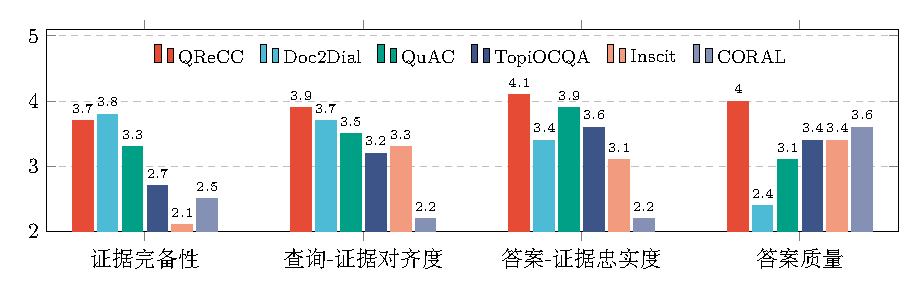
\includegraphics[width=\linewidth]{assets/figs/quality-asses.pdf}

    \bicaption{不同数据集上对多个强大的开源大语言模型进行平均定量分析结果}{Average quantitative analysis results of multiple powerful open-source LLMs on different datasets using our proposed MTR-EVAL metrics }

    \label{fig:quality-asses}

\end{figure}















人工/混合基准的"稀疏性陷阱"。审计结果显示，QReCC、Doc2Dial、QuAC 等被视为"黄金标准"的人工或半自动数据集，在答案质量与答案-证据忠实度上普遍得分较高。其中，QReCC 在忠实度维度达到 $4.1/5.0$，在查询-证据对齐度上达到 $3.9/5.0$，表明其标注答案在语言学层面较为规范，且与所标文档具备基本的事实对应关系。然而，这些数据集在证据完备性维度上表现显著分化：尽管 Doc2Dial 的完备性评分达到 $3.8$，但 TopiOCQA 与 InSCIT 分别仅为 $2.7$ 与 $2.1$，为所有基准中的最低值。这一现象直接印证了人工标注在大规模语料中难以避免的认知边界局限：标注者基于单一文档逆向构造查询，缺乏全局扫描能力，导致大量等效正例被遗漏（即 $\hat{G}_i \setminus G_i \neq \emptyset$）。在检索评估中，这种稀疏性会直接转化为假阴性惩罚，使现代稠密检索器的真实性能被系统性低估。


全自动基准的"对齐性崩塌"。与人工基准形成鲜明对比，CORAL 等依赖静态层级规则的合成基准在查询-证据对齐度上表现显著劣化，评分低至 $2.2/5.0$，同时其答案-证据忠实度也仅为 $2.2/5.0$，为所有基准中的最低值。CORAL 合成的数据中，其生成的查询常常与标注的支撑文档存在严重的语义错位（相关分析参见附录\ref{app:coral_audit}）。例如，数据集中首条样本的查询涉及“天体地质动力学预测方法”，而其标注的支撑文档却详细论述“DOI 标识符系统的技术架构”。这种结构性错位暴露出缺乏全局验证的启发式合成易产生系统性噪声：静态文档标题树无法约束动态用户意图，导致“结构驱动”取代“语义驱动”。这一现象深刻表明：自动化方法虽突破了人力成本瓶颈，但若未引入全局判别测试与多智能体制衡，其产出的数据信噪比难以满足严谨评估需求。



四维指标的协同诊断价值。图~\ref{fig:quality-asses} 进一步揭示了单一指标评估的局限性。以 Doc2Dial 为例，其在证据完备性上得分较高（$3.8$），但在答案质量上仅为 $2.4$，反映出该数据集在标注完整性与语言学规范性之间存在显著张力。类似地，QuAC 在忠实度（$3.9$）与完备性（$3.3$）上表现均衡，但查询-证据对齐度（$3.5$）仍有提升空间。这种多维度的质量画像表明，对话检索基准的评估不能依赖单一指标，而需通过四维体系的协同作用实现精准诊断。高完备性但低对齐度的数据集可能导致检索模型在开放域场景下的性能被高估；而高忠实度但低质量的答案则可能误导生成模块的优化方向。


评估指标的"可靠性系数"意义。综合审计结果揭示了一个关键推论：在 MTR-Eval 综合评分较低的基准上取得高 Recall/NDCG 分数，其实际学术价值有限。因为高分可能源于模型对噪声文档的偶然匹配（$G_i \setminus \hat{G}_i$），或对稀疏金标的过拟合（$\hat{G}_i \setminus G_i$）。反之，仅在 MTR-Eval 高分基准上表现优异的检索系统，才具备真实的语义建模与上下文推理能力。MTR-Eval 因此不仅是一套诊断工具，更应被视为检索评估的 \textbf{前置可靠性过滤器（Pre-requisite Reliability Filter）}。未来对话检索研究必须将基准质量审计纳入标准流程，盲目追求在低质量基准上的指标提升将导致研究方向的系统性偏离。通过量化诊断历史基准的质量鸿沟，MTR-Eval 为后续高保真合成确立了可微分的优化目标，彻底推动对话检索评估从"局部启发式"迈向"全局感知自动化"新范式。







\section{本章小结}



本章阐述了 MTR-Eval 基准质量评估方法的设计逻辑、实现机制与实证效果。针对现有对话检索基准中金标文档集 $G_i$ 与真实证据集 $\hat{G}_i$ 之间的质量鸿沟，本文构建了覆盖查询-证据对齐度、证据完备性、答案-证据忠实度与答案质量的四维细粒度评估体系，分别从集合论角度形式化定义了标注噪声与稀疏性的检测逻辑，并提出了基于判别性测试的代理任务协议。为克服单一 LLM 评估的自偏好与指令敏感性，本章设计了异构多模型集成策略与逐点评分去偏机制，通过 7 款前沿开源模型的统计聚合有效稀释了特定架构的生成偏好与位置偏差。



验证实验表明，该方法与人类专家判断高度一致（Pearson 相关系数达 0.74--0.89，$p \ll 0.001$），且判别性测试代理任务在人工复核中展现出 98\% 的召回精度（Fleiss' Kappa $\kappa = 0.92$），充分证实了其作为数据集“可靠性系数”的科学性与可复现性。通过对 QReCC等历史基准的量化审计，本章揭示了人工标注的认知边界局限与自动化合成的对齐性缺陷，确立了“高质量基准是检索评估前提”的核心论断，为对话检索研究提供了标准化的诊断标尺。



本章提出的评估协议不仅实现了对基准数据质量的精准量化与去偏重打分，更以可微分的质量目标为后续数据合成框架的设计提供了理论指引。下一章将详细论述 MTR-Pipeline 多智能体合成流水线的构建机制，重点阐述如何基于 MTR-Eval 的审计反馈，结合贪心遍历聚类算法与角色制衡协议，实现从“局部启发式标注”向“全局感知自动化合成”的范式跨越。